% !TEX root = BA-Bericht.tex
 % TODO Anhänge anfügen
% Wir haben dies jeweils über \chapter gelöst
% \includepdf[pages=-]{PDF-ANHANG}


% TODO Anhänge anfügen
% Wir haben dies jeweils über \chapter gelöst
% \includepdf[pages=-]{PDF-ANHANG}


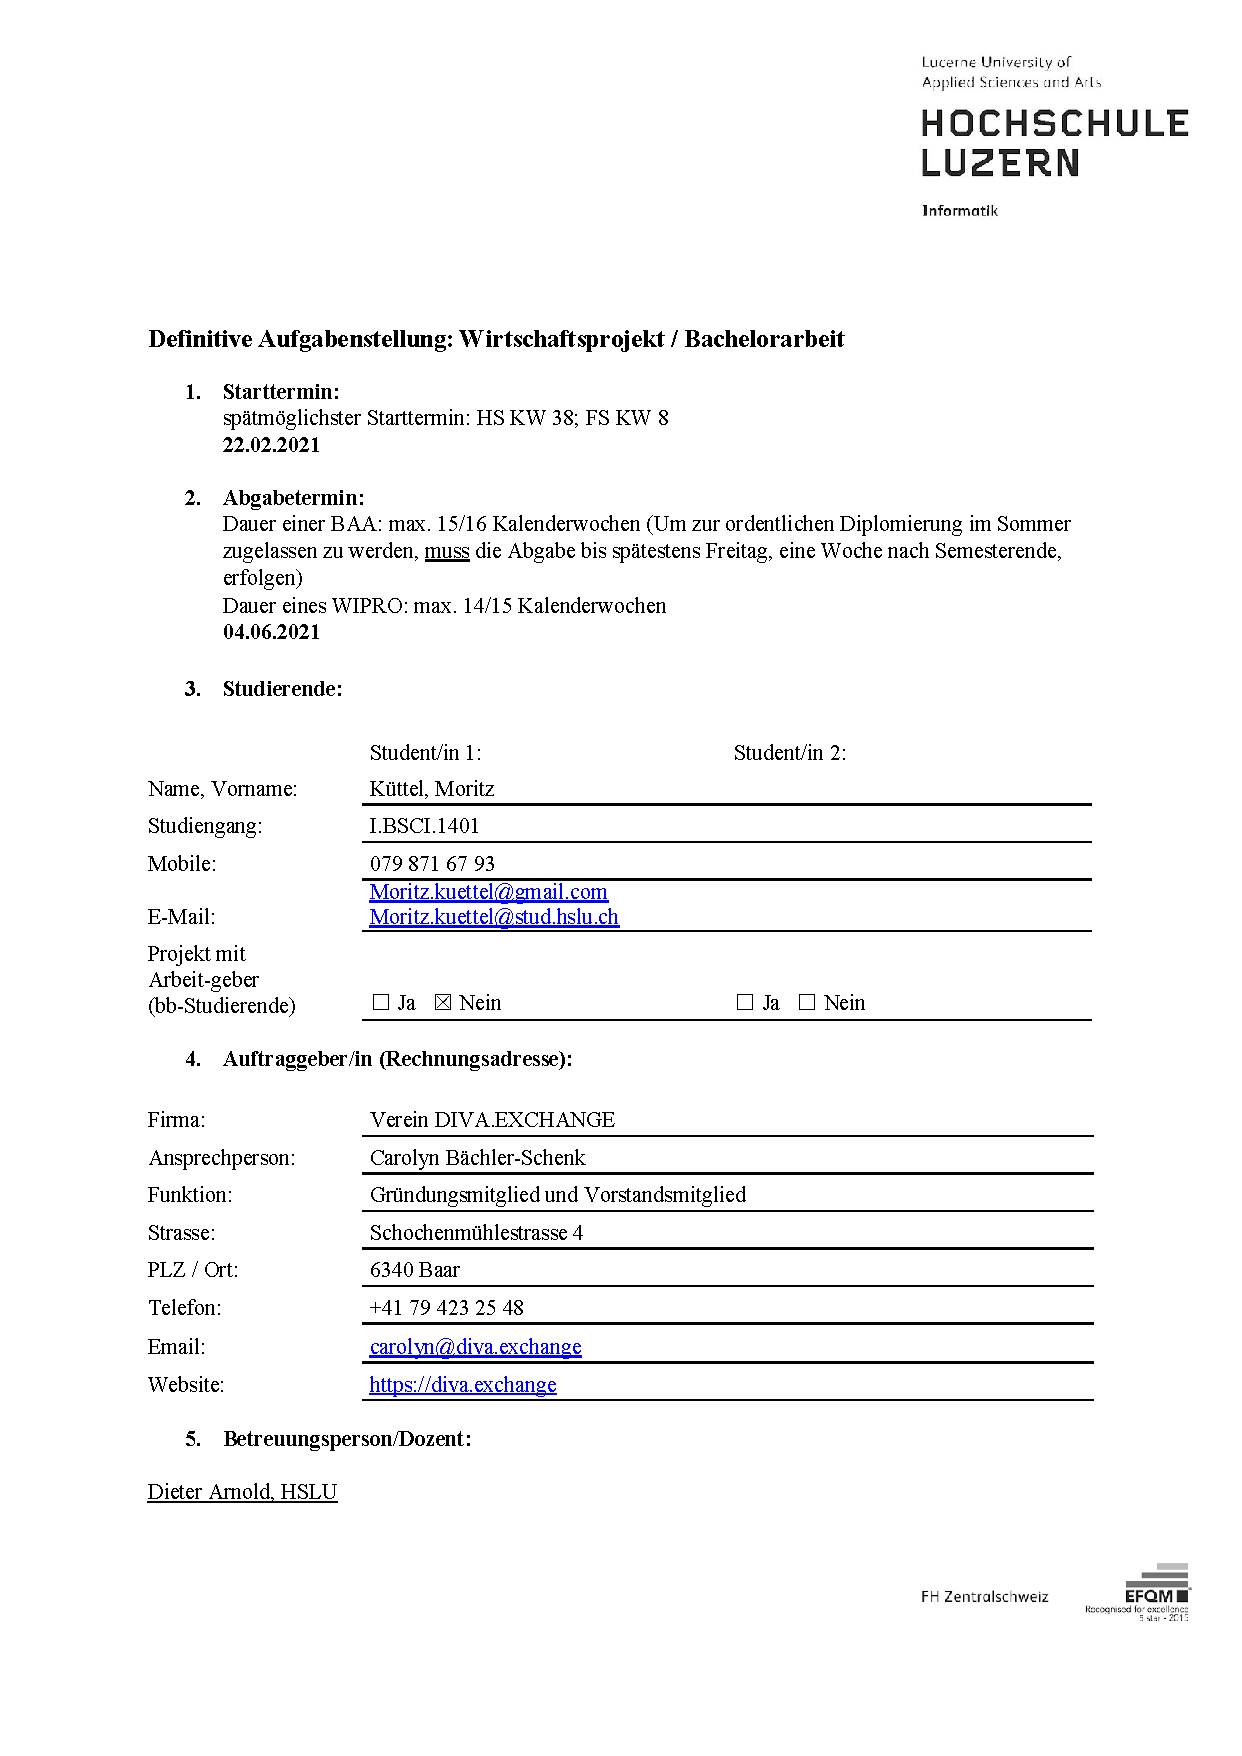
\includepdf[
     addtotoc={1,chapter,0,Aufgabenstellung,ch:aufgabenstellung},
     pages=-
]{include/129_BAA_Aufgabenstellung.pdf}

\chapter{Resultate}

Die folgende Tabelle~\fullref{tab:resultate} beschreibt Resultate und Unterresultate die während dieser Bachelorarbeit erarbeitet werden sollen.
Diese Tabelle wurde zu Beginn des Projekts zusammengestellt anhand der Anforderungen im Abschnitt~\ref{sec:Anforderungen}.
 Diese Liste von Resultaten wurde aus Planungsgründen erstellt, um etwa einschätzen zu können, wie viel Aufwand welche Teile der Arbeit mit sich bringen und den Umfang abzugrenzen.
Jedes Resultat hat einen eindeutigen Identifier in  der Spalte ''Nr'' aufgelistet.
Die Spalte ``Anforderung'' bezieht sich darauf, welche Anforderungen für das jeweilige Resultat massgebend sind.
In der letzten Spalte ''Geschätzter Arbeitsaufwand'', wurde zu beginn des Projekts abgeschätzt wie viel Arbeitsaufwand (in Stunden) das Resultat verursacht.

\begin{longtable}{p{0.8cm} l p{3.5cm} p{2cm}}
    \toprule
    \bfseries Nr & \bfseries Resultat & \bfseries Anforderung& \multicolumn{1}{p{3cm}}{\bfseries Geschätzter Arbeitsaufwand} \\
    \midrule \endhead
    D            & \textbf{Dokumentation}                                       & \reqref{DOCS} & \textbf{Total 44h}  \\
    \midrule                                                               
    D.1          & \; Dokumenten Layout                                &       & 8h   \\
    D.2          & \; Aufbau des Berichts                              &       & 4h   \\
    D.3          & \; Titelseite                                       &       & 2h   \\
    D.4          & \; Zusammenfassung / Abstract                       &       & 2h   \\
    D.5          & \; Einleitung                                       &       & 4h   \\
    D.6          & \; Beschreibung Motivation / Problem                &       & 2h   \\
    D.7          & \; Beschreibung der Aufgabenstellung                &       & 2h   \\
    D.8          & \; Beschreibung der Ziele / Vision                  &       & 1h   \\
    D.9          & \; Fragestellungen / Hypothesen                     &       & 2h   \\
    D.11         & \; Reflektion / Fazit                               &       & 3h   \\
    D.12         & \; Persönliches Projektfazit                        &       & 1h   \\
    D.13         & \; Ausblick                                         &       & 4h   \\
    D.14         & \; Anhang                                           &       & 3h   \\
    D.15         & \; Zwischenpräsentation                             & \reqref{PRES}  & 6h  \\
    \midrule                                                               
    R            & \textbf{Recherche}                                           & \reqref{SDTF} \reqref{DOCS}  & \textbf{Total 40h} \\
    \midrule                                                               
    R.1          & \; Literatur sammeln (Recherche)                    &       & 12h  \\
    R.2          & \; Bibliographie erstellen                          &       &  4h  \\
    R.3          & \; P2P Networks                                     &       &  2h  \\
    R.3.1        & \;   - Latenz / Bandbreite / Performanz             &       &  2h  \\
    R.4          & \; Beschreibung I2P                                 &       & 10h  \\
    R.4.1        & \; -- Begrifflichkeiten                              &       &  4h  \\
    R.4.2        & \; -- Funktionsweise                                 &       &  2h  \\
    R.4.3        & \; -- Bandbreite                                     &       &  2h  \\
    R.4.4        & \; -- Latenz                                         &       &  2h  \\
    R.5          & \; Deployment von Testnetzwerken                    &       &  4h  \\
    R.6          & \; Beschreibung der Wissenschaftlichen Methode      &       &  2h  \\
    R.7          & \; Metriken für die Auswertung                      & \reqref{TPER} \reqref{TISO} \reqref{TREP}  &  6h  \\
    \midrule                                                               
    K            & \textbf{Testkonzept          }                               & \reqref{TKON} \reqref{DOCS}  & \textbf{Total 46h}  \\
    \midrule                                                               
    K.1          & \; Beschreibung Ideen / Konzepte                    &       &  4h  \\
    K.2          & \; Anforderungen an den Teststand                   &       &  4h  \\
    K.3          & \; Teststrategie                                    &       &  4h  \\
    K.4          & \; Architektur Teststand                            &       &  4h  \\
    K.5          & \; Komponentendiagramm                              &       &  2h  \\
    K.6          & \; Beschreibung was gemessen werden soll            &       &  8h  \\
    K.7.1        & \; -- Bandbreite                                     & \reqref{TLIM} &  2h  \\
    K.7.1        & \; -- Anzahl Tunnels                                 & \reqref{TCNF}    &  2h  \\
    K.7.1        & \; -- Latenz von Nachrichten                         & \reqref{TLAT}    &  2h  \\
    K.7.1        & \; -- Ressourcenauslastung eines Knotens             & \reqref{TPER}    &  2h  \\
    K.8          & \; Beschreibung wie gemessen wird                   &       & 10h  \\
    K.8.1        & \; -- Isolation des Netzwerks                        & \reqref{ORDR}    &  2h  \\
    K.8.1        & \; -- Verschiedene Netzwerksegmente                  & \reqref{ORDR}    &  2h  \\
    K.8.2        & \; -- Latenz                                         & \reqref{ORDR}    &  2h  \\
    K.8.3        & \; -- Bandbreite                                     &       &  2h  \\
    K.8.4        & \; -- Konfigurationsmöglichkeiten                    & \reqref{TCNF} &  2h  \\
    K.9.5        & \; \glsname{ci}                                     & \reqref{TVRS} &  6h  \\
    K.9.6        & \; Beschreibung der Auswertungsmethode              &               &  4h  \\
    \midrule                                                               
    I            & \textbf{Teststand Design und Implementation}                 & \reqref{TINF} \reqref{DOCS} & \textbf{Total 124h} \\
    \midrule
    I.1          & \; Software Design                                  &       &  16h \\
    I.1          & \; Implementation                                   &       &  72h \\
    I.2.1        & \; -- Deployment des Testnetzwerkes                  & \reqref{TVRS} \reqref{TPER} &  8h \\
    I.2.2        & \; -- Netzwerksegmentierung                          & \reqref{TISO} &  8h \\
    I.2.3        & \; -- Konfigurationsmöglichkeiten                    & \reqref{TCNF} &  8h \\
    I.2.4        & \; -- Skalierung                                     & \reqref{TSCL} &  8h \\
    I.2.5        & \; -- Bandbreitenbeschränkung                        & \reqref{TLIM} &  8h \\
    I.2.6        & \; -- Reproduzierbarkeit                             & \reqref{TREP} &  8h \\
    I.2.7        & \; -- Latenzmessung                                  & \reqref{TLAT} &  8h \\
    I.2.8        & \; -- Messung der Ressourcenauslastung               & \reqref{TPER} &  8h \\
    I.2.9        & \; -- Verschiedene Testaufbauten                     & \reqref{TVRS} &  8h \\
    I.3          & \; Test des Labors                                  &       &  24h \\
    I.4          & \; Handbuch für den Teststand                       &       &  12h \\
    I.4.1        & \; -- Installation                                   &       &   2h \\
    I.4.3        & \; -- Konfiguration                                  &       &   2h \\
    I.4.3        & \; -- Ausführen von Messungen                        &       &   2h \\
    I.4.3        & \; -- Beschreibung der gesammelten Messdaten         &       &   4h \\
    I.4.3        & \; -- Beispiele                                      &       &   2h \\
    \midrule                                                                        
    A            & \textbf{Messung und Auswertung}                              & \reqref{EVAL} \reqref{DOCS}   & \textbf{Total 52h}  \\
    \midrule
    A.1          & \; Sammlung an Messdaten für die Auswertung         &        &  12h  \\
    A.2          & \; Beschreibung der Auswertungsmethode              &        &   4h  \\
    A.3          & \; Auswertung der Messungen                         &                    & 20h  \\
    A.3.1        & \; -- Einfluss der Knoten auf die Latenz             & \reqref{TLAT}      &  6h  \\
    A.3.2        & \; -- Einfluss der Anzahl Verbindungen auf die Latenz& \reqref{TLAT} \reqref{TLIM} &  6h  \\
    A.3.3        & \; -- Einfluss der Bandbreite auf Latenz             & \reqref{TLAT} \reqref{TLIM} &  6h  \\
    A.3.4        & \; -- Äussere Einflüsse / Unreinheiten               & \reqref{TREP} \reqref{TISO} &  2h  \\
    A.4          & \; Verschiedene Diagramme/Grafiken                  &       &  8h  \\
    A.5          & \; Auswertung der Anforderungen an den Teststand    & \reqref{TINF} &  4h  \\
    A.6          & \; Zusammenfassung der Auswertung                   &       &  4h  \\
    \midrule                                                               
    P            & \textbf{Project Management Dokumentation}                    & \reqref{DOCS} \reqref{ITER}  &  \textbf{Total 54h}  \\
    \midrule
    P.1          & \; Beschreibung Projektorganisation                 &       &  1h  \\
    P.3          & \; Projektmanagement Methode                        &       &  2h  \\
    P.2          & \; Beschreibung Projektumfang                       &       &  2h  \\
    P.4          & \; Projektplanung                                   &       &  8h  \\
    P.5          & \; Liste von Requirements                           &       &  4h  \\
    P.6          & \; Liste von Resultaten                             &       &  4h  \\
    P.9          & \; Arbeitsjournal                                   &       &  4h  \\
    P.10         & \; Meeting-Protokolle und Notizen                   &       & 29h  \\
    \midrule                                                               
                 & \bfseries  Geschätzter Arbeitsaufwand               & \textbf{Total} & \bfseries 360h \\
    \midrule
    \bottomrule
    \caption{Resultate}
    \label{tab:resultate}
\end{longtable}

\chapter{Meeting-Notizen}
\label{ch:meetingnotes}


\includepdf[
    addtotoc={1,section,1,Notizen  Kick-Off-Meeting 24.02.2021,sec:meeting_24_02_2021},
    pages=-
]{Meetings/24-02-2021.pdf}

\includepdf[
    addtotoc={1,section,1,Meeting-Notizen 26.02.2021,sec:meeting_26_02_2021},
    pages=-
]{Meetings/26-02-2021.pdf}

\includepdf[
    addtotoc={1,section,1,Meeting-Notizen 03.03.2021 9:30,sec:meeting_03_03_2021},
    pages=-
]{Meetings/03-03-2021.pdf}


\includepdf[
    addtotoc={1,section,1,Meeting-Notizen 03.03.2021 14:00,sec:meeting_03_03_2021},
    pages=-
]{Meetings/03-03-2021-1400.pdf}


\includepdf[
    addtotoc={1,section,1,Meeting-Notizen 05.03.2021,sec:meeting_05_03_2021},
    pages=-
]{Meetings/05-03-2021.pdf}


\includepdf[
    addtotoc={1,section,1,Meeting-Notizen 10.03.2021,sec:meeting_10_03_2021},
    pages=-
]{Meetings/10-03-2021.pdf}

\includepdf[
    addtotoc={1,section,1,Meeting-Notizen 12.03.2021,sec:meeting_12_03_2021},
    pages=-
]{Meetings/12-03-2021.pdf}

\includepdf[
    addtotoc={1,section,1,Meeting-Notizen 24.03.2021,sec:meeting_24_03_2021},
    pages=-
]{Meetings/24-03-2021.pdf}

\includepdf[
    addtotoc={1,section,1,Meeting-Notizen 31.03.2021,sec:meeting_31_03_2021},
    pages=-
]{Meetings/31-03-2021.pdf}

\includepdf[
    addtotoc={1,section,1,Meeting-Notizen 14.04.2021,sec:meeting_14_04_2021},
    pages=-
]{Meetings/14-04-2021.pdf}

\includepdf[
    addtotoc={1,section,1,Zwischenpräsentation 21.04.2021,sec:meeting_21_04_2021},
    pages=-
]{Meetings/21-04-2021.pdf}


\clearpage% Flush earlier floats (otherwise order might not be correct)
\begin{landscape}% Landscape page
\chapter{Journal}
\label{sec:journal}

    Die folgende Tabelle \fullref{tab:journal} listet die geleisteten Stunden für diese Bachelorarbeit auf. Jede Zeile beinhaltet einen Task und ist unter umständen mit einem oder mehreren Issues auf codeberg.org verbunden.

    \scriptsize

    \begin{longtable}{r l r r r p{2.2cm} p{4.5cm} p{4.5cm} }
        \toprule
        \bfseries Datum & \bfseries Ort & \bfseries Von &
        \bfseries Bis & \bfseries Stunden &
        \bfseries Issue \# & \bfseries Task & \bfseries Notizen \\
        \midrule

        \endhead{}

        \csvreader[
            late after line=\\\midrule,
            late after last line=\\\midrule,
        ]{include/journal.csv}{}
        {\csvlinetotablerow}

       \csvreader[
           head to column names,
           late after line=\\\midrule,
           late after last line=\\\bottomrule,
         ]{include/journal-total-hours.csv}{}
         {& & \bfseries Total (Ist)  & \bfseries hours & \Hours{} \\
          & & \bfseries Total (Soll) & \bfseries hours & 360:00
         }
        \caption{Journal}\label{tab:journal}
    \end{longtable}

\end{landscape}
\clearpage% Flush page



% \chapter{Other Markdown stuff?}
% \label{ch:OtherMarkdownStuff}
% \markdownInput[shiftHeadings=1]{include/somwhere/something.md}

